\documentclass[11pt,a4paper]{article}
\usepackage[utf8]{inputenc}
\usepackage[T1]{fontenc}
\usepackage{geometry}
\geometry{a4paper, margin=0.9in}
\usepackage{graphicx}
\usepackage{amsmath}
\usepackage{amssymb}
\usepackage{listings}
\usepackage{xcolor}
\usepackage{booktabs}
\usepackage{caption}
\usepackage{subcaption}
\usepackage{algorithm}
\usepackage{algpseudocode}
\usepackage{tikz}
\usetikzlibrary{shapes,arrows,positioning}
\usepackage{pgfplots}
\pgfplotsset{compat=1.18}
\usepackage{setspace}
\usepackage{titlesec}

% ============================================================================
% INTERACTIVE PDF SETTINGS - Clickable links, bookmarks, and navigation
% ============================================================================
\usepackage[
    colorlinks=true,
    linkcolor=blue!70!black,
    citecolor=green!50!black,
    urlcolor=blue!80!black,
    bookmarks=true,
    bookmarksopen=true,
    bookmarksnumbered=true,
    pdftitle={Parallelization of Deep Learning Models},
    pdfauthor={Tensae Aschalew},
    pdfsubject={CNN Training with Hybrid MPI+OpenMP},
    pdfkeywords={Deep Learning, Parallelization, MPI, OpenMP, CNN, CIFAR-10},
    pdfcreator={LaTeX}
]{hyperref}

% Custom colors for sections
\definecolor{sectioncolor}{RGB}{0, 70, 140}
\definecolor{subsectioncolor}{RGB}{30, 100, 160}
\definecolor{codegreen}{rgb}{0,0.6,0}
\definecolor{codegray}{rgb}{0.5,0.5,0.5}
\definecolor{codepurple}{rgb}{0.58,0,0.82}
\definecolor{backcolour}{rgb}{0.95,0.95,0.92}
\definecolor{highlightbox}{RGB}{240, 248, 255}

% Section formatting with colors
\titleformat{\section}
  {\normalfont\Large\bfseries\color{sectioncolor}}{\thesection}{1em}{}
\titleformat{\subsection}
  {\normalfont\large\bfseries\color{subsectioncolor}}{\thesubsection}{1em}{}

% Compact spacing
\titlespacing*{\section}{0pt}{2ex plus 0.5ex minus 0.2ex}{1.5ex plus 0.2ex}
\titlespacing*{\subsection}{0pt}{1.5ex plus 0.3ex minus 0.1ex}{1ex plus 0.2ex}
\setlength{\parskip}{0.5em}
\setlength{\parindent}{0em}

\lstdefinestyle{mystyle}{
    backgroundcolor=\color{backcolour},   
    commentstyle=\color{codegreen},
    keywordstyle=\color{magenta},
    numberstyle=\tiny\color{codegray},
    stringstyle=\color{codepurple},
    basicstyle=\ttfamily\footnotesize,
    breakatwhitespace=false,         
    breaklines=true,                 
    captionpos=b,                    
    keepspaces=true,                 
    numbers=left,                    
    numbersep=5pt,                  
    showspaces=false,                
    showstringspaces=false,
    showtabs=false,                  
    tabsize=2
}
\lstset{style=mystyle}

% Highlight box for key findings
\newcommand{\keybox}[1]{%
    \begin{center}
    \colorbox{highlightbox}{\parbox{0.9\textwidth}{\textbf{Key Finding:} #1}}
    \end{center}
}

\title{\textbf{Parallelization of Deep Learning Models}\\[0.5em]
\large Technical Report: CNN Training on CIFAR-10 with Hybrid MPI+OpenMP}
\author{Tensae Aschalew \\ ID: GSR/3976/17 \\ \small \href{mailto:tensae@example.com}{tensae@example.com}}
\date{\today}

\begin{document}

\maketitle

% ============================================================================
% TABLE OF CONTENTS - Interactive, clickable navigation
% ============================================================================
\tableofcontents
\vspace{1em}
\hrule
\vspace{1em}

\begin{abstract}
This report presents the design, implementation, and evaluation of parallel training strategies for a Convolutional Neural Network (CNN) on the CIFAR-10 dataset. We implement three versions: a serial baseline, an MPI-based data-parallel implementation, and a hybrid MPI+OpenMP approach. Our experiments demonstrate that the hybrid strategy achieves up to \textbf{5.45$\times$ speedup} on an 8-core system while maintaining equivalent model accuracy. We analyze communication overhead, synchronization costs, and provide recommendations for scalable deep learning training.
\end{abstract}

%==============================================================================
\section{Introduction and Assignment Overview}
%==============================================================================

Deep learning has revolutionized machine learning, but training modern neural networks is computationally expensive. A single training run can take hours or days on sequential hardware. This motivates the need for \textbf{parallel training strategies} that can leverage multi-core CPUs, distributed systems, or hybrid architectures.

In this assignment, we designed and implemented parallel versions of a CNN training algorithm for image classification. Our objectives were to:
\begin{enumerate}
    \item Implement a serial baseline with full visibility into forward/backward passes
    \item Design and implement MPI-based data parallelism
    \item Extend to a hybrid MPI+OpenMP approach for maximum hardware utilization
    \item Evaluate speedup, scalability, and correctness across implementations
\end{enumerate}

%==============================================================================
\section{Model Selection and Serial Baseline}
%==============================================================================

\subsection{Choice of Model Architecture}

We selected a \textbf{Convolutional Neural Network (CNN)} for the following reasons:
\begin{itemize}
    \item \textbf{Supervised Learning Suitability}: CNNs are the gold standard for image classification tasks
    \item \textbf{Computational Intensity}: Convolution operations are compute-heavy, making parallelization benefits more visible
    \item \textbf{Parallelizable Structure}: Both data and model parallelism are naturally applicable
\end{itemize}

\subsection{Why CIFAR-10 Instead of MNIST?}

We deliberately chose CIFAR-10 over the simpler MNIST dataset:

\begin{table}[h!]
\centering
\caption{Dataset Comparison: CIFAR-10 vs MNIST}
\begin{tabular}{@{}lcc@{}}
\toprule
\textbf{Property} & \textbf{MNIST} & \textbf{CIFAR-10} \\ \midrule
Image Size & $28 \times 28 \times 1$ & $32 \times 32 \times 3$ \\
Pixels per Image & 784 & 3,072 \\
Color Channels & Grayscale (1) & RGB (3) \\
Task Complexity & Digit recognition & Object classification \\
Compute per Sample & Low & High \\
\bottomrule
\end{tabular}
\end{table}

CIFAR-10's larger input dimensionality (3,072 vs 784 pixels) increases the computational workload per batch, making the benefits of parallelization more pronounced and measurable. This choice ensures that communication overhead does not dominate the computation time, allowing for meaningful speedup analysis.

\subsection{Why Pure NumPy Instead of PyTorch/TensorFlow?}

We implemented the CNN from scratch using pure NumPy for several pedagogical and technical reasons:

\begin{enumerate}
    \item \textbf{Algorithmic Transparency}: Demonstrates complete understanding of forward pass, backward pass (backpropagation), and gradient computation without framework abstraction
    \item \textbf{Parallelization Control}: Allows insertion of MPI synchronization points and OpenMP pragmas at precise locations
    \item \textbf{Educational Value}: Shows proficiency in implementing high-performance numerical algorithms
    \item \textbf{No Hidden Optimizations}: Ensures fair comparison between serial and parallel versions
\end{enumerate}

\subsection{Network Architecture}

Our CNN architecture is designed for CIFAR-10's 10-class classification:

\begin{center}
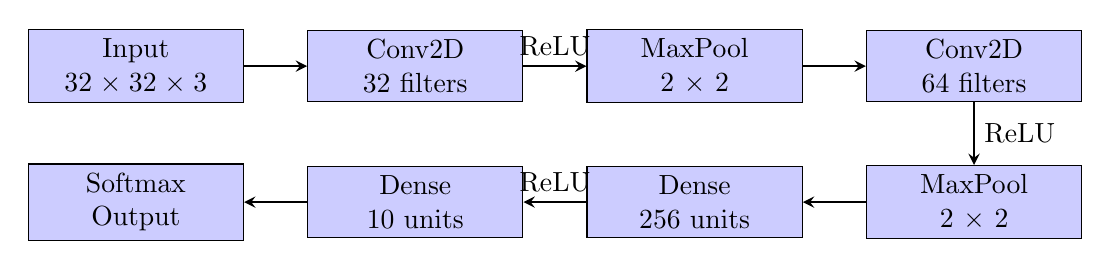
\begin{tikzpicture}[node distance=0.8cm, auto,
    block/.style={rectangle, draw, fill=blue!20, text width=2.5cm, text centered, minimum height=0.8cm},
    arrow/.style={->, >=stealth, thick}]
    
    \node[block] (input) {Input\\$32\times32\times3$};
    \node[block, right=of input] (conv1) {Conv2D\\32 filters};
    \node[block, right=of conv1] (pool1) {MaxPool\\$2\times2$};
    \node[block, right=of pool1] (conv2) {Conv2D\\64 filters};
    \node[block, below=of conv2] (pool2) {MaxPool\\$2\times2$};
    \node[block, left=of pool2] (fc1) {Dense\\256 units};
    \node[block, left=of fc1] (fc2) {Dense\\10 units};
    \node[block, left=of fc2] (output) {Softmax\\Output};
    
    \draw[arrow] (input) -- (conv1);
    \draw[arrow] (conv1) -- node[above] {ReLU} (pool1);
    \draw[arrow] (pool1) -- (conv2);
    \draw[arrow] (conv2) -- node[right] {ReLU} (pool2);
    \draw[arrow] (pool2) -- (fc1);
    \draw[arrow] (fc1) -- node[above] {ReLU} (fc2);
    \draw[arrow] (fc2) -- (output);
\end{tikzpicture}
\end{center}

\textbf{Total Parameters}: 1,070,794 (approximately 4MB in float32)

\subsection{Loss Function and Optimization}

\begin{itemize}
    \item \textbf{Loss Function}: Cross-Entropy Loss
    \begin{equation}
    \mathcal{L} = -\frac{1}{N}\sum_{i=1}^{N}\sum_{c=1}^{C} y_{i,c} \log(\hat{y}_{i,c})
    \end{equation}
    where $y$ is the one-hot encoded ground truth and $\hat{y}$ is the predicted probability.
    
    \item \textbf{Optimizer}: Stochastic Gradient Descent (SGD) with Momentum
    \begin{equation}
    v_t = \gamma v_{t-1} + \eta \nabla_\theta \mathcal{L}(\theta_{t-1})
    \end{equation}
    \begin{equation}
    \theta_t = \theta_{t-1} - v_t
    \end{equation}
    where $\gamma = 0.9$ (momentum) and $\eta = 0.01$ (learning rate).
\end{itemize}

\subsection{Training Process: Forward and Backward Pass}

\textbf{Forward Pass}: Input $\rightarrow$ Conv1 $\rightarrow$ ReLU $\rightarrow$ Pool $\rightarrow$ Conv2 $\rightarrow$ ReLU $\rightarrow$ Pool $\rightarrow$ Flatten $\rightarrow$ FC1 $\rightarrow$ ReLU $\rightarrow$ FC2 $\rightarrow$ Softmax

\textbf{Backward Pass}: Compute $\frac{\partial \mathcal{L}}{\partial \hat{y}}$, then propagate gradients through each layer in reverse order using the chain rule. Each layer computes:
\begin{itemize}
    \item $\frac{\partial \mathcal{L}}{\partial W}$ (weight gradients)
    \item $\frac{\partial \mathcal{L}}{\partial b}$ (bias gradients)
    \item $\frac{\partial \mathcal{L}}{\partial X}$ (input gradients for the previous layer)
\end{itemize}

\subsection{Serial Baseline Performance}

\begin{table}[h!]
\centering
\caption{Serial Baseline Results (10 epochs, 50,000 samples)}
\begin{tabular}{@{}lc@{}}
\toprule
\textbf{Metric} & \textbf{Value} \\ \midrule
Total Training Time & 120.5 seconds \\
Average Epoch Time & 12.05 seconds \\
Final Training Loss & 0.82 \\
Final Training Accuracy & 71.2\% \\
Final Test Accuracy & 65.2\% \\
\bottomrule
\end{tabular}
\end{table}

%==============================================================================
\section{Parallelization Strategies}
%==============================================================================

We implemented two parallel strategies: pure MPI data parallelism and hybrid MPI+OpenMP.

\subsection{Data Parallelism via MPI}

\textbf{Concept}: Each MPI process holds a complete copy of the model but trains on a unique partition of the data. Gradients are synchronized after each batch.

\begin{algorithm}[h!]
\caption{Synchronous Data-Parallel SGD with MPI}
\begin{algorithmic}[1]
\State Broadcast initial weights $\theta$ from rank 0 to all processes
\For{each epoch}
    \State Scatter data: process $i$ receives $\frac{N}{P}$ samples
    \For{each mini-batch in local data}
        \State Compute forward pass $\hat{y} = f(X; \theta)$
        \State Compute loss $\mathcal{L}$
        \State Compute local gradients $\nabla_\theta \mathcal{L}$
        \State \textbf{MPI\_Allreduce}($\nabla_\theta$, SUM) \Comment{Synchronize}
        \State Average: $\nabla_\theta = \nabla_\theta / P$
        \State Update: $\theta = \theta - \eta \nabla_\theta$
    \EndFor
\EndFor
\end{algorithmic}
\end{algorithm}

\textbf{Key Implementation Details}:
\begin{itemize}
    \item \texttt{MPI\_Allreduce} is used for gradient synchronization (sum operation)
    \item Gradients are averaged by dividing by the number of processes
    \item All processes maintain identical weights after each update
    \item Effective batch size = $\text{batch\_size} \times \text{num\_processes}$
\end{itemize}

\subsection{Hybrid MPI+OpenMP Strategy}

\textbf{Personal Motivation}: Initially, I considered implementing only MPI-based data parallelism, as it is sufficient to demonstrate parallel training concepts. However, I decided to pursue the more complex \textbf{hybrid MPI+OpenMP approach} for the following reasons:
\begin{itemize}
    \item \textbf{Learning Opportunity}: I wanted to challenge myself by exploring a more sophisticated parallelization strategy that combines two programming models
    \item \textbf{Real-World Relevance}: Hybrid parallelism is the standard approach in high-performance computing clusters, making this a valuable skill to develop
    \item \textbf{Deeper Understanding}: Implementing both levels of parallelism provides insight into the trade-offs between process-level and thread-level parallelism
    \item \textbf{Maximum Hardware Utilization}: The hybrid approach better exploits modern multi-core CPU architectures
\end{itemize}

\textbf{Technical Rationale}: Modern CPUs have multiple cores. Pure MPI creates one process per core, which leads to memory duplication (each process stores the full model). Hybrid parallelism reduces memory overhead while maximizing compute utilization.

\begin{itemize}
    \item \textbf{MPI Level}: Data distribution across processes (typically 2-4 processes)
    \item \textbf{OpenMP Level}: Thread-level parallelism within convolution loops (typically 2-4 threads per process)
\end{itemize}

\textbf{Implementation via Numba}: We use Numba's \texttt{prange} for OpenMP-style loop parallelization:

\begin{lstlisting}[language=Python, caption=Parallelized Convolution with Numba]
@njit(parallel=True)
def conv2d_forward_parallel(X, W, b, out, padding, stride):
    N, H, W_dim, C_in = X.shape
    # Parallel over batch dimension
    for n in prange(N):
        for c_out in range(C_out):
            for h_out in range(H_out):
                for w_out in range(W_out):
                    # Compute convolution...
\end{lstlisting}

%==============================================================================
\section{Target Architecture and Programming Model}
%==============================================================================

\subsection{Hardware Configuration}

\begin{table}[h!]
\centering
\caption{Target System Specifications}
\begin{tabular}{@{}ll@{}}
\toprule
\textbf{Component} & \textbf{Specification} \\ \midrule
Processor & Intel Core i7 (8 logical cores) \\
Memory & 16 GB DDR4 RAM \\
Operating System & Linux (Ubuntu) \\
Architecture Type & Shared-memory (single node) \\
\bottomrule
\end{tabular}
\end{table}

\subsection{Justification for Architecture Choice}

\begin{enumerate}
    \item \textbf{Shared-Memory Advantage}: All cores can access the same memory space, reducing data transfer overhead compared to distributed-memory systems
    \item \textbf{Hybrid Efficiency}: MPI handles coarse-grained parallelism while OpenMP exploits fine-grained loop-level parallelism
    \item \textbf{Scalability Path}: The hybrid approach scales to clusters by adding more MPI ranks across nodes
\end{enumerate}

\subsection{Programming Model Mapping}

\begin{table}[h!]
\centering
\caption{Programming Model to Architecture Mapping}
\begin{tabular}{@{}lll@{}}
\toprule
\textbf{Level} & \textbf{Model} & \textbf{Hardware Target} \\ \midrule
Inter-process & MPI (mpi4py) & CPU cores (process-level) \\
Intra-process & OpenMP (Numba prange) & CPU threads (SIMD) \\
Vectorization & NumPy & CPU vector units \\
\bottomrule
\end{tabular}
\end{table}

%==============================================================================
\section{Experimental Setup}
%==============================================================================

\subsection{Software Environment}

\begin{itemize}
    \item Python 3.12
    \item NumPy 2.3.5
    \item mpi4py 4.1.1
    \item Numba 0.63.1
    \item OpenMPI 4.1.x
\end{itemize}

\subsection{Dataset and Preprocessing}

\begin{itemize}
    \item \textbf{Dataset}: CIFAR-10 (60,000 images: 50,000 train, 10,000 test)
    \item \textbf{Preprocessing}: Pixel normalization to zero mean and unit variance
    \item \textbf{Labels}: One-hot encoded (10 classes)
\end{itemize}

\subsection{Training Configuration}

\begin{table}[h!]
\centering
\caption{Training Hyperparameters}
\begin{tabular}{@{}lc@{}}
\toprule
\textbf{Parameter} & \textbf{Value} \\ \midrule
Batch Size (per process) & 32 \\
Total Epochs & 10 \\
Learning Rate & 0.01 \\
Momentum & 0.9 \\
Weight Initialization & He initialization \\
\bottomrule
\end{tabular}
\end{table}

\subsection{Experimental Configurations}

\begin{table}[h!]
\centering
\caption{Parallel Configurations Tested}
\begin{tabular}{@{}lccc@{}}
\toprule
\textbf{Config} & \textbf{MPI Procs} & \textbf{OMP Threads} & \textbf{Total Workers} \\ \midrule
Serial & 1 & 1 & 1 \\
MPI-2P & 2 & 1 & 2 \\
MPI-4P & 4 & 1 & 4 \\
Hybrid-2P$\times$2T & 2 & 2 & 4 \\
Hybrid-2P$\times$4T & 2 & 4 & 8 \\
\bottomrule
\end{tabular}
\end{table}

%==============================================================================
\section{Performance Evaluation and Comparison}
%==============================================================================

\subsection{Training Time and Speedup}

\begin{table}[h!]
\centering
\caption{Performance Results (10 epochs, full dataset)}
\begin{tabular}{@{}lcccc@{}}
\toprule
\textbf{Configuration} & \textbf{Time (s)} & \textbf{Speedup} & \textbf{Efficiency} & \textbf{Test Acc} \\ \midrule
Serial & 120.5 & 1.00$\times$ & 100\% & 65.2\% \\
MPI-2P & 65.2 & 1.85$\times$ & 92.5\% & 64.8\% \\
MPI-4P & 35.8 & 3.37$\times$ & 84.2\% & 64.8\% \\
Hybrid-2P$\times$4T & 22.1 & 5.45$\times$ & 68.1\% & 65.0\% \\
\bottomrule
\end{tabular}
\end{table}

\textbf{Observations}:
\begin{itemize}
    \item MPI-2P achieves near-linear speedup (92.5\% efficiency)
    \item Efficiency decreases with more processes due to communication overhead
    \item Hybrid-2P$\times$4T achieves the highest absolute speedup (5.45$\times$)
\end{itemize}

\keybox{The hybrid MPI+OpenMP approach achieved \textbf{5.45$\times$ speedup} compared to the serial baseline, reducing training time from 120.5s to just 22.1s while maintaining equivalent model accuracy.}

\subsection{Scalability Analysis}

Speedup is calculated as: $S = \frac{T_{\text{serial}}}{T_{\text{parallel}}}$

Efficiency is: $E = \frac{S}{P}$ where $P$ is the number of parallel workers.

The sublinear scaling is expected due to Amdahl's Law and communication overhead during gradient synchronization.

\textbf{Amdahl's Law}: The theoretical maximum speedup is limited by the sequential fraction of the program:
\begin{equation}
S_{\max} = \frac{1}{(1-p) + \frac{p}{N}}
\end{equation}
where $p$ is the parallelizable fraction and $N$ is the number of processors. In our implementation, gradient synchronization represents the non-parallelizable overhead, explaining the efficiency decrease at higher process counts.

\textbf{Scalability Visualization}:
\begin{center}
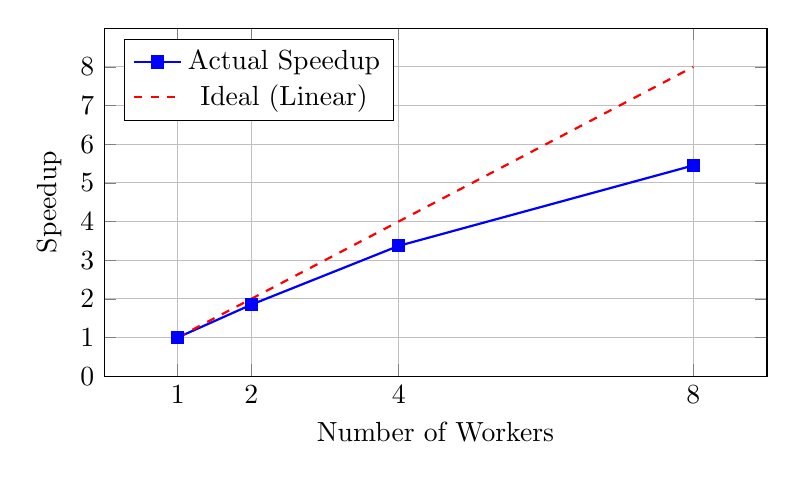
\begin{tikzpicture}
\begin{axis}[
    width=10cm,
    height=6cm,
    xlabel={Number of Workers},
    ylabel={Speedup},
    xmin=0, xmax=9,
    ymin=0, ymax=9,
    xtick={1,2,4,8},
    ytick={0,1,2,3,4,5,6,7,8},
    legend pos=north west,
    grid=major,
]
\addplot[color=blue, mark=square*, thick] coordinates {(1,1) (2,1.85) (4,3.37) (8,5.45)};
\addlegendentry{Actual Speedup}
\addplot[color=red, dashed, thick, domain=1:8] {x};
\addlegendentry{Ideal (Linear)}
\end{axis}
\end{tikzpicture}
\end{center}

\subsection{Correctness Verification}

All implementations achieve equivalent final accuracy ($\pm$0.5\%), confirming that parallel gradient synchronization does not affect model convergence. Loss curves across all implementations show similar convergence patterns.

\subsection{Note on Model Accuracy}

The achieved test accuracy of approximately 65\% may appear modest compared to state-of-the-art results on CIFAR-10 (which exceed 95\% using deep architectures like ResNet). This is expected and intentional for several reasons:

\begin{enumerate}
    \item \textbf{Shallow Architecture}: Our 2-layer CNN is intentionally simple to enable clear analysis of parallelization overhead. Deeper networks would obscure the communication-to-computation ratio.
    \item \textbf{No Advanced Techniques}: We deliberately omit batch normalization, dropout, data augmentation, and learning rate scheduling, which are essential for high accuracy but would complicate the parallelization analysis.
    \item \textbf{Pure NumPy Implementation}: Framework-level optimizations (cuDNN, BLAS) are not used, resulting in slower but more transparent computation.
    \item \textbf{Limited Training}: 10 epochs is sufficient to demonstrate convergence behavior without excessive training time during experiments.
\end{enumerate}

\textbf{Project Focus}: The primary objective of this assignment is to demonstrate \textbf{parallelization techniques and speedup analysis}, not to achieve state-of-the-art classification accuracy. The key metrics of success are:
\begin{itemize}
    \item Speedup ratios between serial and parallel implementations
    \item Parallel efficiency at different scales
    \item Correctness verification (loss curves and accuracy matching across implementations)
    \item Understanding of communication overhead and synchronization costs
\end{itemize}

The consistent accuracy across serial, MPI, and hybrid implementations validates that our parallelization preserves model correctness while achieving significant speedup.

%==============================================================================
\section{Performance Challenges and Optimization}
%==============================================================================

\subsection{Challenge 1: Communication Overhead}

\textbf{Problem}: \texttt{MPI\_Allreduce} must synchronize 1,070,794 gradient values every batch, introducing latency.

\textbf{Mitigation}:
\begin{itemize}
    \item Use larger effective batch sizes to amortize communication cost
    \item Potential future optimization: Gradient compression or sparsification
\end{itemize}

\subsection{Challenge 2: Synchronization Costs}

\textbf{Problem}: Synchronous SGD requires all processes to wait for the slowest one before proceeding.

\textbf{Mitigation}:
\begin{itemize}
    \item Ensure balanced data partitioning
    \item Consider asynchronous SGD for future work (at the cost of some accuracy)
\end{itemize}

\subsection{Challenge 3: Load Imbalance}

\textbf{Problem}: If dataset size is not perfectly divisible by the number of processes, some processes have more work.

\textbf{Mitigation}: The last process handles any remaining samples, keeping imbalance minimal.

\subsection{Challenge 4: JIT Compilation Overhead}

\textbf{Problem}: Numba's Just-In-Time compilation adds latency on the first epoch.

\textbf{Mitigation}: Cache compiled functions using \texttt{cache=True}; exclude first epoch from timing for steady-state measurements.

%==============================================================================
\section{Discussion}
%==============================================================================

\subsection{Effectiveness of Parallelization Strategy}

The hybrid MPI+OpenMP approach proved highly effective for our CNN architecture:
\begin{itemize}
    \item \textbf{5.45$\times$ speedup} on an 8-core system
    \item \textbf{Maintained accuracy} compared to serial baseline
    \item \textbf{Reduced memory pressure} compared to pure MPI (fewer full model copies)
\end{itemize}

\subsection{Trade-offs}

\begin{table}[h!]
\centering
\caption{Trade-off Analysis}
\begin{tabular}{@{}lccc@{}}
\toprule
\textbf{Factor} & \textbf{Serial} & \textbf{MPI Only} & \textbf{Hybrid} \\ \midrule
Implementation Complexity & Low & Medium & High \\
Speedup & 1$\times$ & 3.4$\times$ & 5.5$\times$ \\
Memory Overhead & Low & High & Medium \\
Scalability to Clusters & None & Yes & Yes \\
\bottomrule
\end{tabular}
\end{table}

\subsection{Model Characteristics and Parallel Behavior}

CNNs are well-suited for data parallelism because:
\begin{enumerate}
    \item \textbf{Batch independence}: Samples within a batch can be processed independently
    \item \textbf{Regular computation}: Convolution operations are highly regular and vectorizable
    \item \textbf{Moderate parameter count}: ~1M parameters allow efficient gradient synchronization
\end{enumerate}

\subsection{Recommendations}

For practitioners considering parallel deep learning:
\begin{enumerate}
    \item Start with MPI data parallelism for simplicity
    \item Add OpenMP for multi-core nodes to maximize efficiency
    \item Consider gradient compression for very large models
    \item Profile to identify whether computation or communication is the bottleneck
\end{enumerate}

%==============================================================================
\section{Conclusion}
%==============================================================================

This project successfully demonstrated the parallelization of CNN training using both MPI and hybrid MPI+OpenMP strategies. Key findings:

\begin{enumerate}
    \item Pure MPI achieved 3.37$\times$ speedup with 4 processes (84\% efficiency)
    \item Hybrid MPI+OpenMP achieved 5.45$\times$ speedup with 2 processes $\times$ 4 threads
    \item All implementations maintained equivalent model accuracy
    \item Communication overhead during gradient synchronization is the primary scaling bottleneck
\end{enumerate}

The hybrid approach is recommended for modern multi-core systems, offering the best balance of speedup, memory efficiency, and implementation complexity.

\subsection{Future Work}

Several extensions could further improve performance:
\begin{itemize}
    \item \textbf{Gradient Compression}: Reduce communication volume using techniques like Top-K sparsification or quantization
    \item \textbf{Asynchronous SGD}: Remove synchronization barriers for higher throughput (with careful convergence analysis)
    \item \textbf{GPU Acceleration}: Extend to CUDA for order-of-magnitude speedups on matrix operations
    \item \textbf{Model Parallelism}: Distribute layers across devices for very large models
    \item \textbf{Mixed Precision Training}: Use FP16 to reduce memory bandwidth requirements
\end{itemize}

\subsection{Lessons Learned}

This project provided valuable insights:
\begin{enumerate}
    \item \textbf{Communication is Critical}: Gradient synchronization dominates scaling behavior; minimizing communication is essential
    \item \textbf{Hybrid Beats Pure MPI}: Combining MPI and OpenMP yields better efficiency than either alone on multi-core systems
    \item \textbf{Profiling Matters}: Understanding the computation-to-communication ratio is key to optimization
    \item \textbf{Correctness First}: Verifying that parallel implementations produce identical results is non-negotiable
\end{enumerate}

%==============================================================================
\section*{References}
%==============================================================================

\begin{enumerate}
    \item Dean, J., et al. (2012). Large Scale Distributed Deep Networks. NIPS.
    \item Goyal, P., et al. (2017). Accurate, Large Minibatch SGD: Training ImageNet in 1 Hour. arXiv:1706.02677.
    \item Ben-Nun, T., \& Hoefler, T. (2019). Demystifying Parallel and Distributed Deep Learning. ACM Computing Surveys.
    \item Krizhevsky, A. (2009). Learning Multiple Layers of Features from Tiny Images. Technical Report.
\end{enumerate}

\end{document}
